\chapter{Plots}
\begin{figure}[H]
\centering
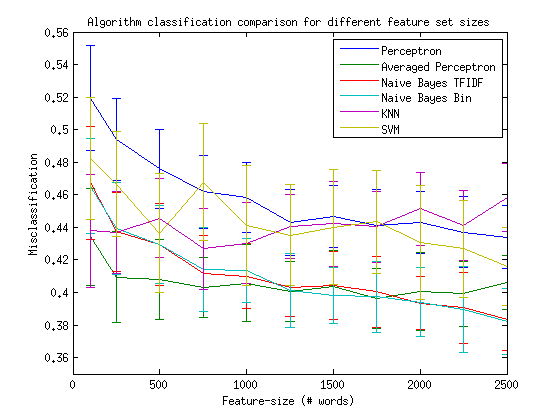
\includegraphics[scale = 1]{../Plottar/feature-size100-2500bigram.png}
\caption{In-domain classification using varying Bigram feature set sizes with 2$\sigma$ height error bars and comparing all algorithms.}
\end{figure} 

\begin{figure}[H]
\centering
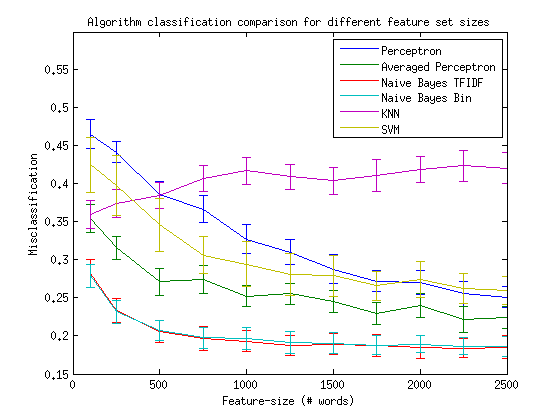
\includegraphics[scale = 1]{../Plottar/feature-size100-2500all.png}
\caption{In-domain sentiment analysis classification error (error bars of height $\sigma$) for the 6 algorithms on varying Unigram feature vector sizes}
\end{figure} 

\begin{figure}[H]
\centering
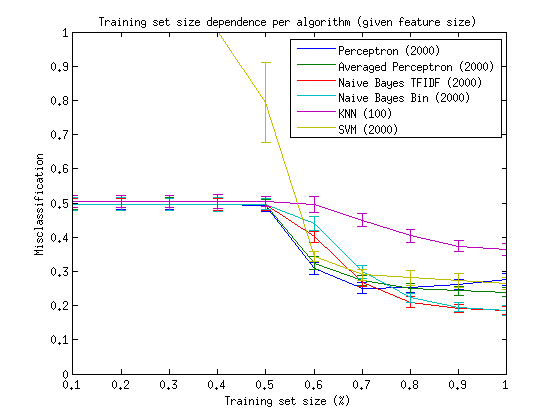
\includegraphics[scale = 1]{../Plottar/training_size_k_2000allknn_100.png}
\caption{Training set size dependence per algorithm}
\end{figure} 

\begin{figure}[H]
\centering
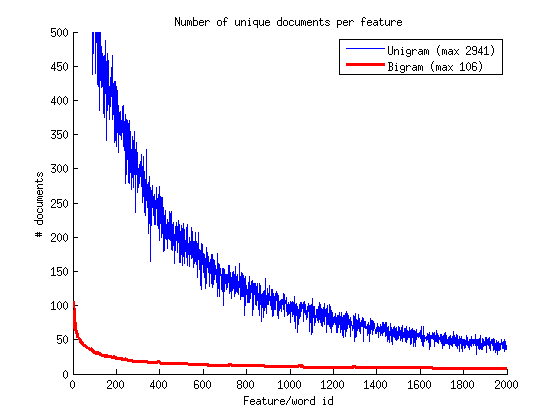
\includegraphics[scale = 1]{../Plottar/documents_per_feature.png}
\caption{Documents per feature. Bigram and Unigram}
\end{figure} 

\begin{figure}[H]
\centering
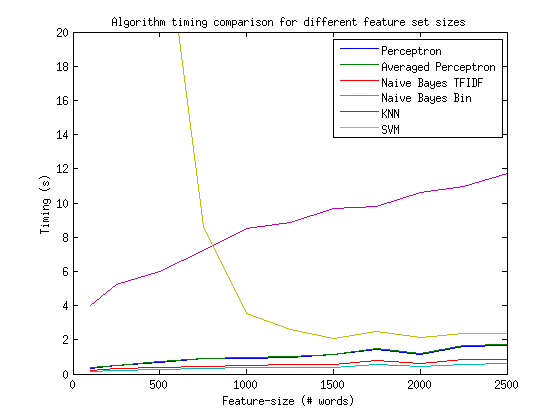
\includegraphics[scale = 1]{../Plottar/feature_size_TIMING.png}
\caption{Timing of different algorithms with different feature sizes}
\end{figure} 

\begin{figure}[H]
\centering
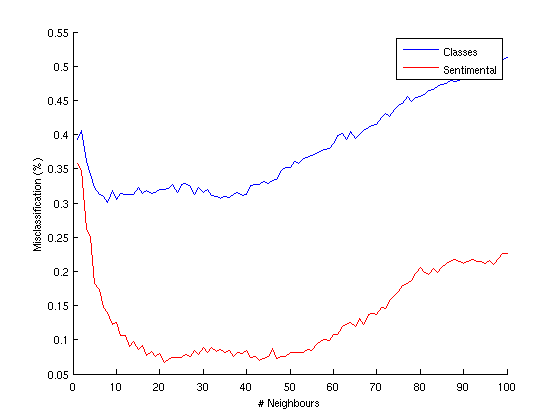
\includegraphics[scale = 1]{../Plottar/knn_2000words_testdata100_unigram.png}
\caption{Different K-values when running KNN on Classes and Sentimental-label}
\end{figure} 


\begin{sidewaysfigure}[H]
\centering
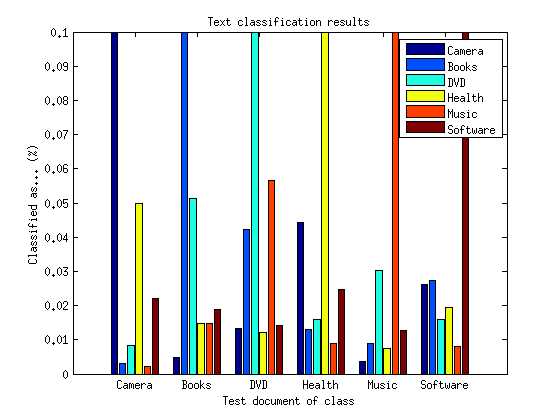
\includegraphics[scale = 0.47]{../Plottar/text_categorization.png}
\caption{Text categorization task}
\end{sidewaysfigure} 


\begin{sidewaysfigure}[H]
\centering
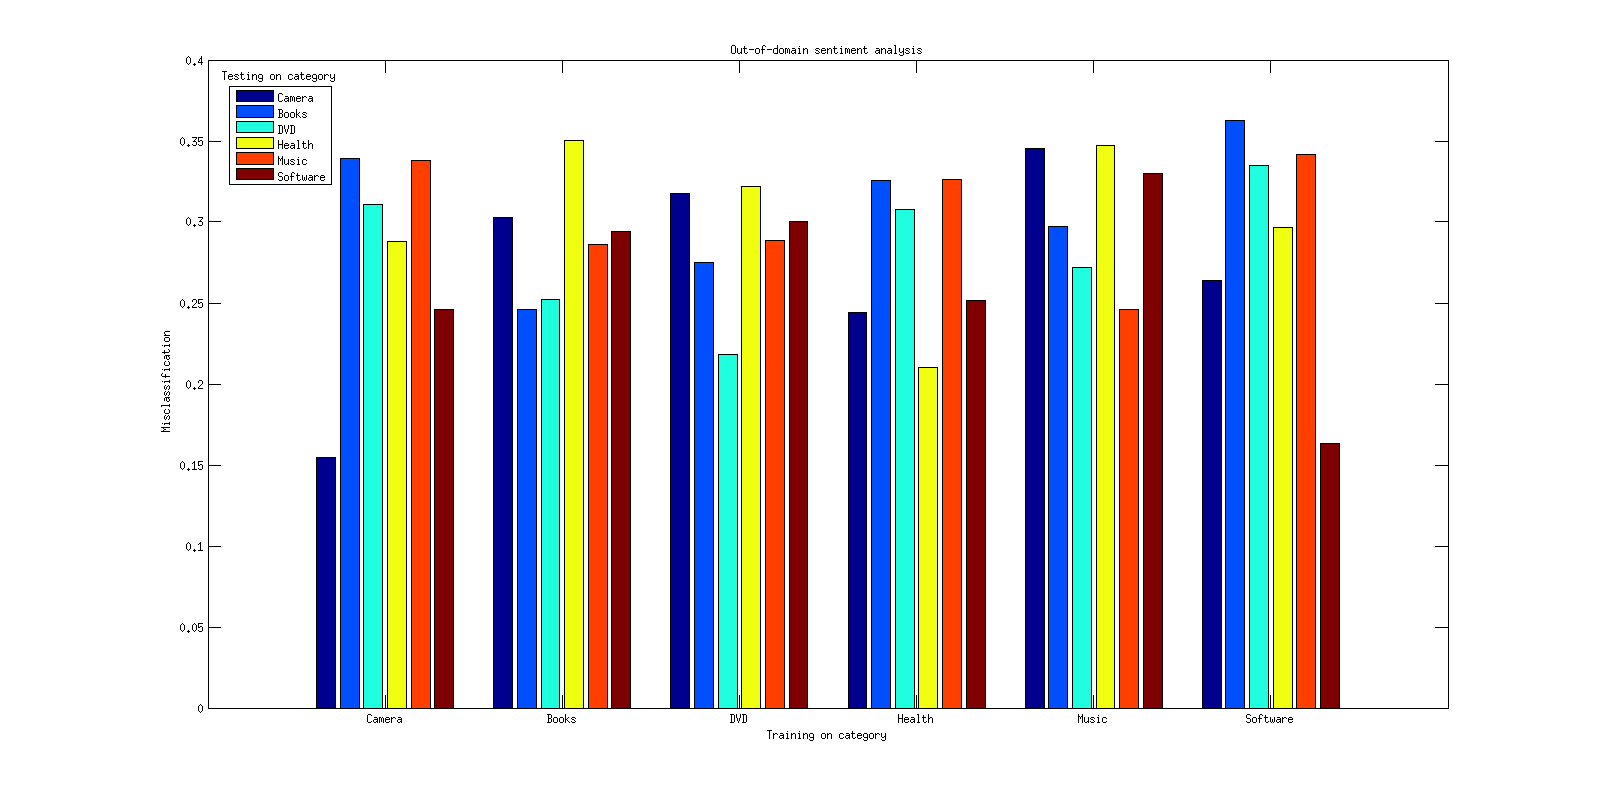
\includegraphics[scale = 0.47]{../Plottar/outofdomain.png}
\caption{Out of domain classification task}
\end{sidewaysfigure} 

\begin{figure}[H]
\centering
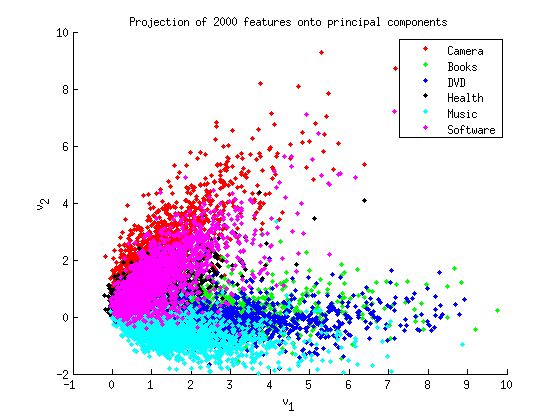
\includegraphics[scale = 1]{../Plottar/pca_all.png}
\caption{PCA on all categories}
\end{figure} 

\begin{figure}[H]
\centering
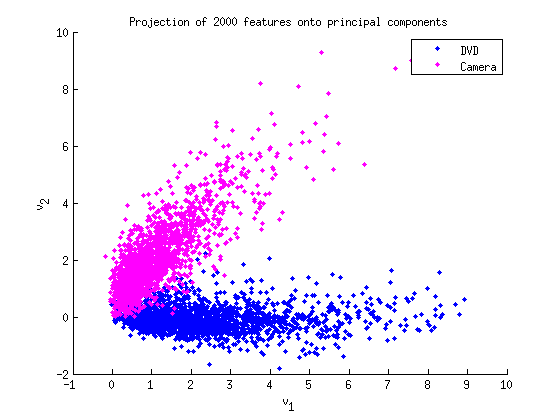
\includegraphics[scale = 1]{../Plottar/pca_nocorr.png}
\caption{PCA on DVD and camera with no correlation}
\end{figure} 

\begin{figure}[H]
\centering
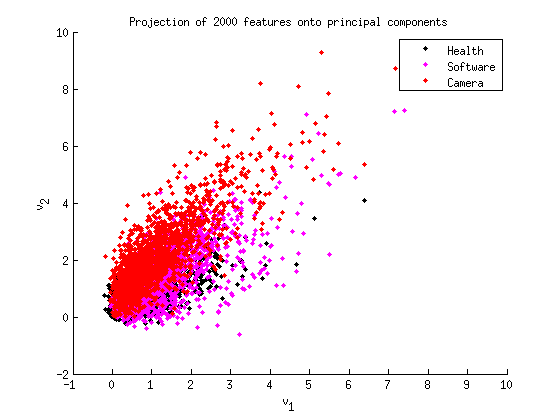
\includegraphics[scale = 1]{../Plottar/pca_largecorr.png}
\caption{PCA on health, software and camera. Represent a large correlation}
\end{figure} 

\begin{figure}[H]
\centering
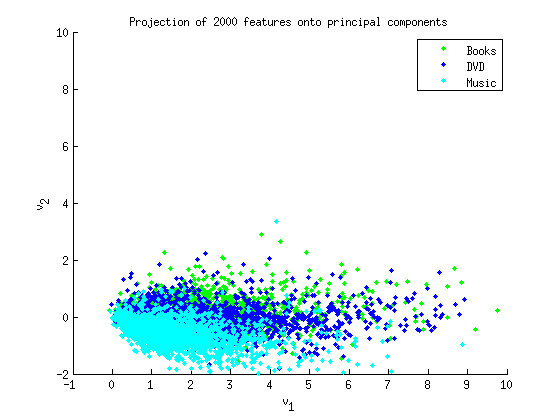
\includegraphics[scale = 1]{../Plottar/pca_somecorr.png}
\caption{PCA on Books, DVD and Music with some correlation}
\end{figure} 

\begin{figure}[H]
\centering
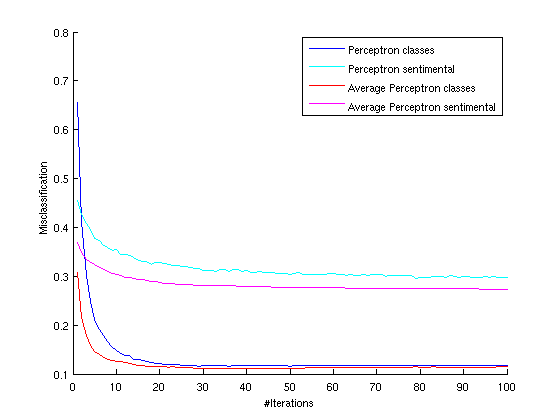
\includegraphics[scale = 1]{../Plottar/perceptron_2000words_unigram_10foldcv_classes-high_sentimental-low.png}
\caption{Different max iteration Perceptron}
\end{figure} 

\chapter{English stop words}
\input{appendix/english_word_stops.txt}

